\documentclass[tikz,border=2pt]{standalone}
\usepackage{amsmath}
\usepackage{amssymb}
\usepackage{pgfplots}
\pgfplotsset{compat=1.18}
\usetikzlibrary{arrows.meta}
\begin{document}
% Sublevel sets L_alpha={2x_1^2+3x_2^2<=alpha} of the convex f(x)=2x_1^2+3x_2^2 for alpha=1,2,4: nested filled ellipses;
% L_4 (Exercise 1.2) has semi-axes sqrt(2) and 2/sqrt(3).
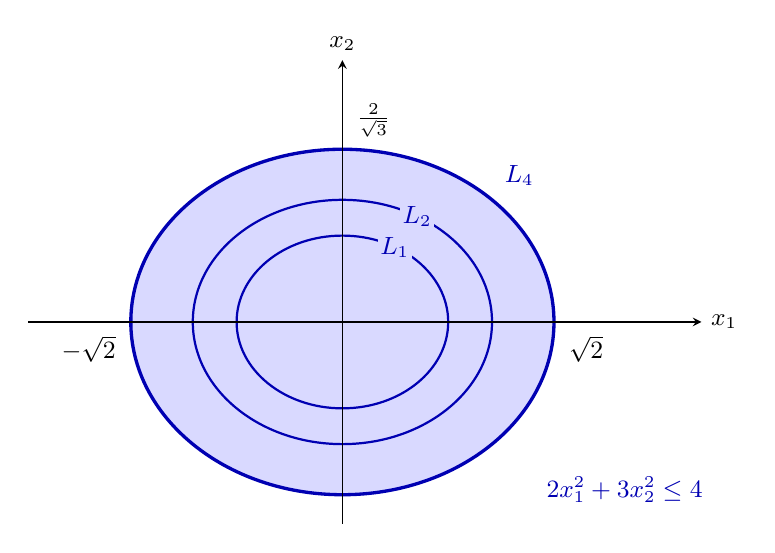
\begin{tikzpicture}[font=\small, >={Latex[length=2mm]}]
  \begin{axis}[
    axis lines=middle, axis on top, xmin=-2.1, xmax=2.4, ymin=-1.35, ymax=1.75,
    xtick=\empty, ytick=\empty,
    xlabel={$x_1$}, ylabel={$x_2$},
    xlabel style={anchor=west}, ylabel style={anchor=south},
    x=1.9cm, y=1.9cm, clip=false
    ]
    \fill[blue!15] (axis cs:0,0) ellipse [x radius=1.41421, y radius=1.1547];
    \draw[blue!70!black, very thick] (axis cs:0,0) ellipse [x radius=1.41421, y radius=1.1547];
    \draw[blue!70!black, thick] (axis cs:0,0) ellipse [x radius=1, y radius=0.8165];
    \draw[blue!70!black, thick] (axis cs:0,0) ellipse [x radius=0.70711, y radius=0.57735];
    \node[blue!70!black, anchor=south west] at (axis cs:1.02,0.85) {$L_4$};
    \node[blue!70!black, fill=blue!15, inner sep=1pt] at (axis cs:0.5,0.707) {$L_2$};
    \node[blue!70!black, fill=blue!15, inner sep=1pt] at (axis cs:0.35,0.5) {$L_1$};
    \node[anchor=north east] at (axis cs:-1.45,-0.03) {$-\sqrt{2}$};
    \node[anchor=north west] at (axis cs:1.45,-0.03) {$\sqrt{2}$};
    \node[anchor=south west] at (axis cs:0.03,1.17) {$\tfrac{2}{\sqrt{3}}$};
    \node[blue!70!black, anchor=west] at (axis cs:1.3,-1.12) {$2x_1^2+3x_2^2\leq4$};
  \end{axis}
\end{tikzpicture}
\end{document}
